\chapter{Preliminary Data and Results}

The research result on identifier renaming has been published in paper ``A Neural Architecture for Detecting Identifier Renaming from Diff'' seen in \autoref{sec:produced-publications}.
This chapter hence presents the preliminary results for the RM2HyperLedger project.

At the current stage, I am evaluating my tool on \cocome. RM2PT first generates JavaFX source code from the requirement document of \cocome, then my program RM2HyperLedger takes over and converts the JavaFX source code to HyperLedger chaincode in Java.

\begin{figure}[ht]
\centering
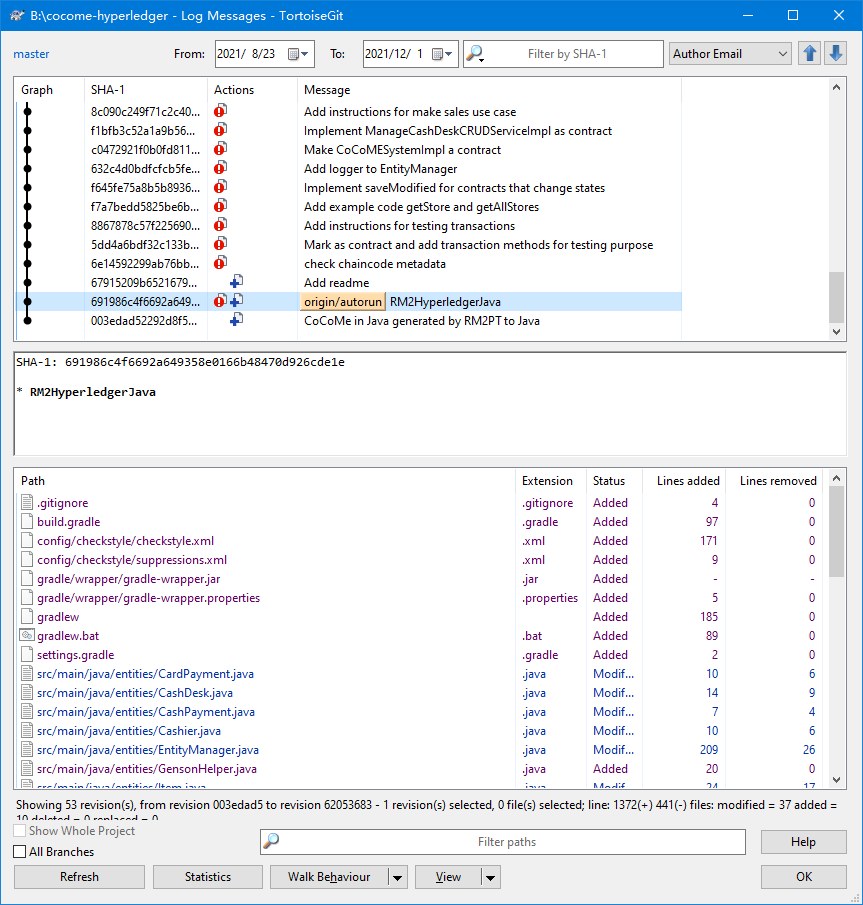
\includegraphics[width=0.9\linewidth]{cocome-hyperledger-log}
\caption{The base of cocome-hyperledger is the JavaFX source code generated by RM2PT. Then RM2HyperLedger automatically converts it to HyperLedger chaincode.}
\label{fig:cocome-hyperledger-log}
\end{figure}

\autoref{fig:cocome-hyperledger-log} shows RM2HyperLedger is able to automatically convert some source code into HyperLedger format, and I have to do more conversions because not all conversion rules have been implemented in RM2HyperLedger. Currently I am collecting my manual conversion rules into RM2HyperLedger, so eventually no manual editing is needed.

Besides the functional implementation, I also worked on requirements validation and test code generation. \autoref{testManageItem} is an example unit test that follows the manage item UML activity diagram. This code ensures all function calls except the last one do not fail, and after each function call, \code{docker stop} stimulates a network node down. Due to the pre- and post-conditions of \code{deleteItem}, this function cannot be called twice, thus reflected in the test code.


\begin{figure}[ht]
\begin{lstlisting}[language=bash, breaklines=true, showstringspaces=false, frame=tb, caption={A Bash function that tests operations in the manage item category}, label=testManageItem]
testManageItem() {
  pci -C mychannel -n cocome --waitForEvent -c '{"function":"ManageItemCRUDServiceImpl:createItem","Args":["1","cookies","10","10","9"]}' || fail

  docker stop "$(docker ps -n 1 --filter 'name=dev' --format '{{.ID}}')"

  peer chaincode query -C mychannel -n cocome -c '{"function":"ManageItemCRUDServiceImpl:queryItem","Args":["1"]}' || fail

  docker stop "$(docker ps -n 1 --filter 'name=dev' --format '{{.ID}}')"

  pci -C mychannel -n cocome --waitForEvent -c '{"function":"ManageItemCRUDServiceImpl:modifyItem","Args":["1","Pepperidge farm cookies","12","5","10"]}' || fail

  docker stop "$(docker ps -n 1 --filter 'name=dev' --format '{{.ID}}')"

  pci -C mychannel -n cocome --waitForEvent -c '{"function":"ManageItemCRUDServiceImpl:deleteItem","Args":["1"]}' || fail

  if pci -C mychannel -n cocome --waitForEvent -c '{"function":"ManageItemCRUDServiceImpl:deleteItem","Args":["1"]}'; then
    fail 'Cannot delete the same item twice'
  fi
}
\end{lstlisting}
\end{figure}

These tests are implemented compatible to GitHub Actions, i.e., GitHub is able to run these tests to verify the correctness of the application. In total, at present three such tests are implemented. \autoref{fig:github-action}~shows one run of these tests on GitHub.

\begin{figure}[ht]
\centering
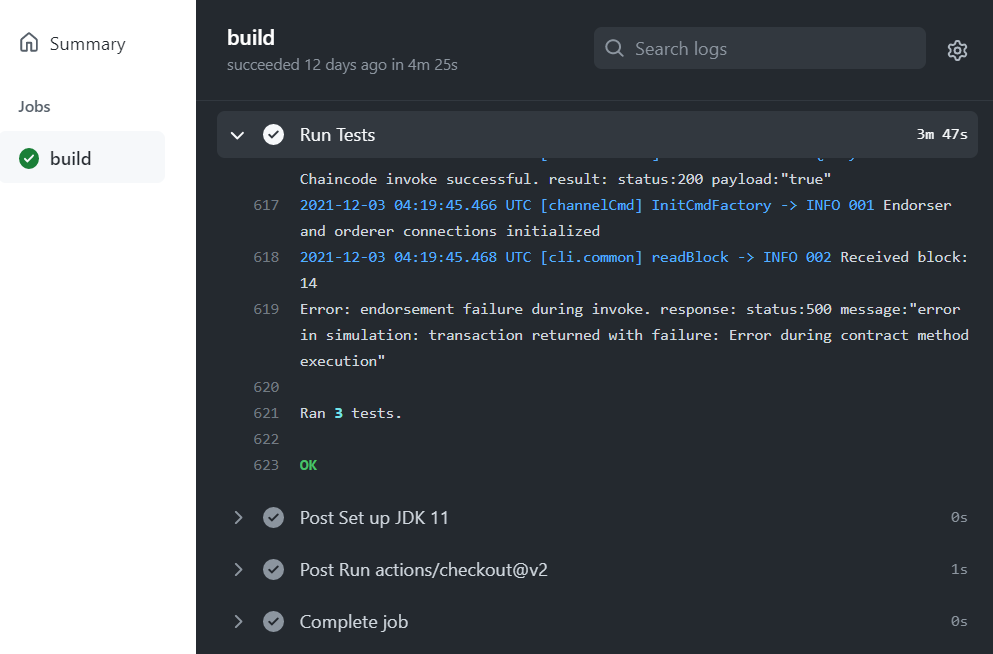
\includegraphics[width=0.9\linewidth]{github-action}
\caption{The code of requirements validation is able to run on GitHub. 3 tests pass.}
\label{fig:github-action}
\end{figure}
